\chapter*{Background}
\addcontentsline{toc}{chapter}{Background}
\section{Literature Review}
In order to understand the design requirements of the library, a literature review needed to be performed. The scope was
narrowed down to 3 systems that showed promise and were broadly representative of the antenna configuration that future
systems would adopt. Most systems will adopt one of the following setups
\begin{enumerate}
    \item Monostatic
    \item Leveled Multistatic
    \item Fully Multistatic
\end{enumerate}
\noindent These terms relate to the position of antennas around the breast tissue and how the resulting scan data would
be structured. \hfill \break

\subsection{MARIA M4}
The first system we will look at is the MARIA M4 system developed by Preece et al within the Electrical and Engineering
Department of the University of Bristol \cite{preeceMARIAM4Clinical2016}. This is the 4th iteration in a series of MARIA systems that evolved from a
system of 16 UWB antennas to 60 antennas in the current system. These all operate in a multistatic configuration,
meaning that any antenna in the array can listen to any other antenna in the array, an example of which can be seen in
Figure \ref{fig:MultistaticExample}. This figure shows a top-down view, however, one can imagine this being generalized
to a hemisphere of antennas around the breast. \hfill

\begin{figure}
    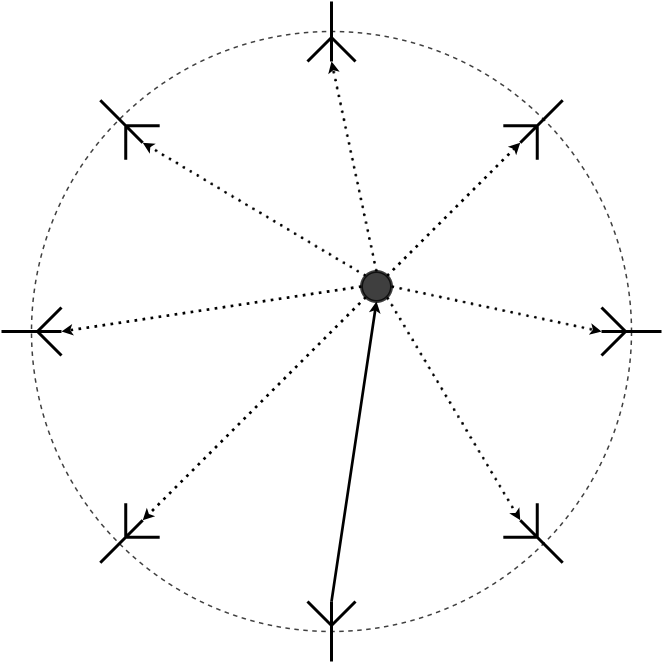
\includegraphics[width=0.3\textwidth]{multistaic.png}
    \centering
    \caption{Example of a Fully Multistatic Configuration (Top-Down)}
    \label{fig:MultistaticExample}
\end{figure}

\noindent As stated before, the MARIA M4 systems makes use of the UWB spectrum over a frequency range of 3.0 to 8.0 GHz. A
VNA was used to step through the frequencies and collect the scans from the antenna. The system exploits the inherent
symmetry in the antenna reciprocity to halve the number of channels (made of a transmitting and receiving antenna)
collected, thereby speeding up the scan time. For the MARIA M4 system, this equates to a 1770 reduction in the number of
channels collected. Figure \ref{fig:MARIAM4}, shows the antenna array used in the M4 system (a), as well as the M5
system (c) which is an integrated package.


\begin{figure}
    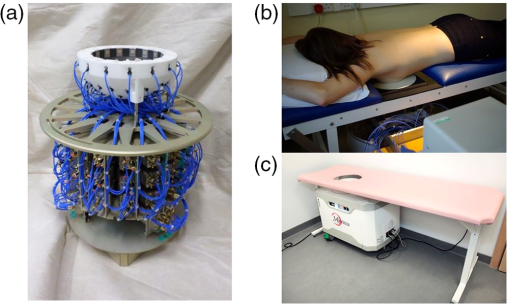
\includegraphics[width=0.5\textwidth]{MARIA_M4.png}
    \centering
    \caption{The MARIA M4 and M5 system. (a) The MARIA M4 antenna array. (b) The M4 in a clinical setting. (c) The integrated M5 package \cite{preeceMARIAM4Clinical2016}}
    \label{fig:MARIAM4}
\end{figure}

\noindent The team scanned 86 participants, with a mean age of 51.4 and a range of 24 - 78 years old. The M4 system showed a sensitivity of
74\% (64/86) when compared with the "gold-standard' of an ultrasound. The "sensitivity" was determined based on the
ability of the M4 system to localize a lesion as it correlated with the location in the ultrasound image. The research
team also divided the group into pre-/peri- and post- menopausal women and found that the sensitivity was 75\% and 73\%
respectively. However, the reliability of these results are called into question when considering the sample size of the
study. Given a sample size of 86, and assuming a normal distribution and that the results are statistically significant
($p < 0.05$, Z = 1.96), a 7.11\% margin of error was calculated. While this may not be enough to conclusively prove
that the M4 system is a viable alternative to Mammograms, it is enough to show promise. With a larger sample size, this
margin of error could be narrowed further.

\subsection{Wavelia}
The second system that was considered was the Wavelia Microwave Breast Imaging System developed by MVG Industries
\cite{moloneyWaveliaMicrowaveBreast2021}. The Wavelia system integrates the imaging system as well as the examination
bed into one complete package (Figure \ref{fig:WaveliaSystem}). The integrated package makes the Wavelia system an
appealing choice for some hospitals, however, its large size may be a barrier to adoption in some facilities where space
is a premium. \hfill \break

\begin{figure}
    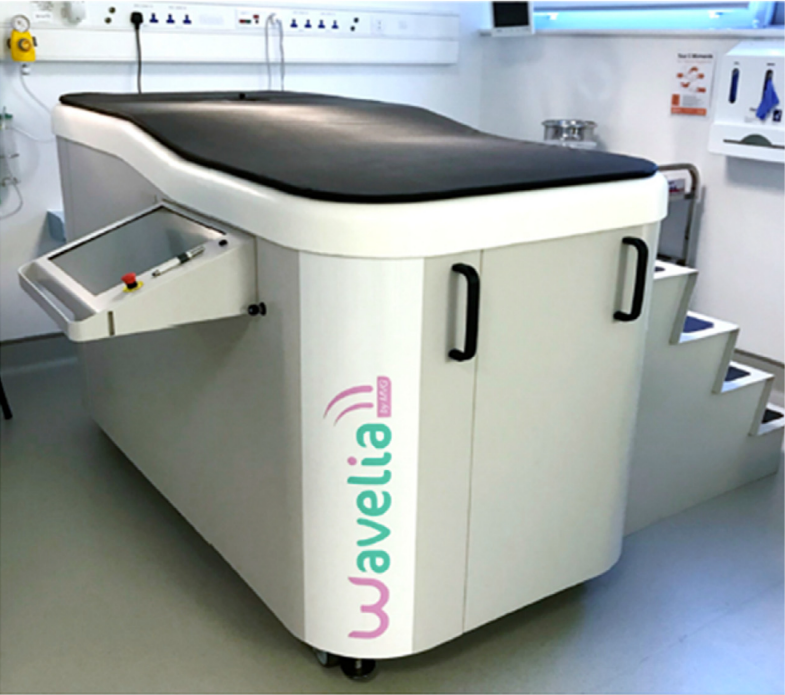
\includegraphics[width=0.5\textwidth]{Wavelia.png}
    \centering
    \caption{The Wavelia System \cite{moloneyWaveliaMicrowaveBreast2021}}
    \label{fig:WaveliaSystem}
\end{figure}

Like in the MARIA M4 system, patients lie in a prone position and place their breasts in the circular cutouts on the
bed. The system then begins to create a 3D reconstruction of the exterior of the breast using a stereoscopic camera.
This also allows for the breast volume to be explicitly calculated rather than being inferred like in the MARIA system.
The Wavelia makes use of the UWB spectrum when imaging the breast, although they opt for a narrower frequency range of
0.5 - 4.0 GHz compared to the 3.0 - 8.0 GHz range of the MARIA system. The antenna configuration, unlike the MARIA system, is an array of 18 Vivaldi-type probes arranged in a concyclic manner
on a horizontal plane. These antennas operate in a Multistatic manner and image the breast in sections parallel to the
coronal plane. The entire antenna assembly moves downwards in 5mm intervals to image the entire breast (Figure \ref{fig:LeveledMultistaticExample}). This is a
leveled multistatic system as opposed to the fully multistatic system in the MARIA M4. This leveled multistatic approach
has the benefit of a theoretically infinite vertical resolution. If the radiologist wanted a finer resolution along the
coronal plane, they would just have to tweak the array vertical step size, rather than having to manufacture an entirely
new antenna array, like in the MERIT system. This leveled approach also allows the parameters of the reconstruction
algorithm to be easily changed based on the particular section of the breast that we are imaging. The fully multistatic
approach, however, would need significant additional logic in the post-processing steps to determine which channels are
coplanar with a particular section. \hfill \break

\begin{figure}
    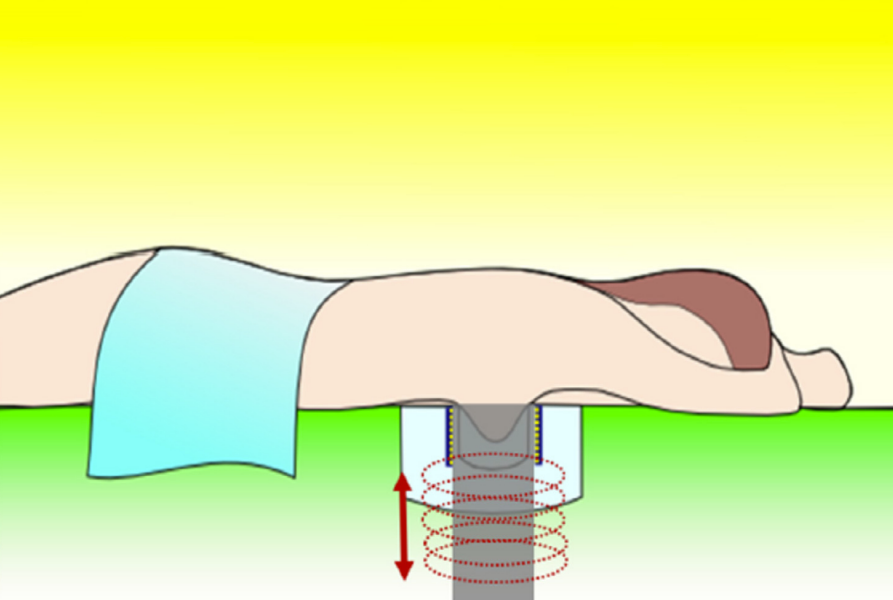
\includegraphics[width=0.5\textwidth]{LeveledMultistatic.png}
    \centering
    \caption{The Leveled Multistatic Approach of Wavelia \cite{moloneyWaveliaMicrowaveBreast2021}}
    \label{fig:LeveledMultistaticExample}
\end{figure}

\noindent The Wavelia paper \cite{moloneyWaveliaMicrowaveBreast2021} conducted a feasibility study on 25 female
participants. While the results aren't statistically significant, they do demonstrate the strengths of the Wavelia
system. 11 of the participants had a biopsy confirmed carcinoma and out of these, the Walia system detected 9 lesions,
with 7 being located to the appropriate region. Overall the system detected an abnormality in 21 of the 24 participants,
leading to a sensitivity of 87.5\%. The researchers do note some limitations of the Walia system, namely it can't detect
any lesions smaller than 10mm. This is significant since the size of the detected lesion plays a big factor when
deciding whether a lesion is cancerous or not. Another limitation of the system is that breast sizes that are too small
cannot be scanned in any great detail by the Wavelia system. Due to the patients being in the prone position, their
breast tissue needs to hang down far enough to have multiple sections of their breast be imaged by the antenna array.
The researchers are working on a subsequent system that should address all the aforementioned limitations. Overall the
participants had a positive outlook on the system. 23 out of the 25 women said that they would recommend the procedure
to other women and all of the women agreed that the information provided was clear and well understood.

\subsection{TSAR}
The third and final system considered for the project was the TSAR system \cite{e.c.fearMicrowaveBreastImaging2013}. Standing for Tissue Sensing Adaptive Radar,
this system was developed by the University of Calgary to address some of the shortcomings of the previous two systems.
In the MERIT and Wavelia systems, reflections from the skin can muddy the data and can lead to artifacts in the final
image. In order to get around this, both systems take an additional scan, offset by a fixed rotational amount in the
coronal plane. The idea being, that any reflections that appear on the first scan would appear with similar amplitude in
the second scan at the same time position, while the tumor would show in a different place, provided that the tumor
doesn't lie on the axis of rotation. This method is known as Rotational Subtraction
\cite{klemmImprovedDelayandSumBeamforming2008}. The TSAR system, on the other hand, makes use of an adaptive algorithm
that instead estimates the skin response at an antenna as the weighted sum of the responses from the neighboring
antennas. This skin response can then be subtracted from the current antenna to remove the reflection artifacts
\cite{makladNeighborhoodBasedAlgorithmFacilitate2012}. \hfill \break

Like the previous two systems, patients lie in the prone position on the examination table, with their breast being
submerged in an immersion liquid. However, unlike the previous two systems, the TSAR operates in a monostatic
configuration. In this setup, there is only one antenna that acts as both the transmitting and the receiving antenna.
This antenna, usually fixed on some type of rotating apparatus, would rotate around the breast to image a section. It
would then step vertically by a fixed amount and repeat the previous step, eventually imaging the entire breast. The
TSAR system also operates on a much wider section of the UWB spectrum, from 50 MHz to 15 GHz, with the frequency data
being collected by a VNA. The system also makes use of a laser in order to help with the 3D reconstruction of the breast
during post-processing. The prototype setup can be seen in Figure \ref{fig:TSARPrototype} \hfill \break

\begin{figure}
    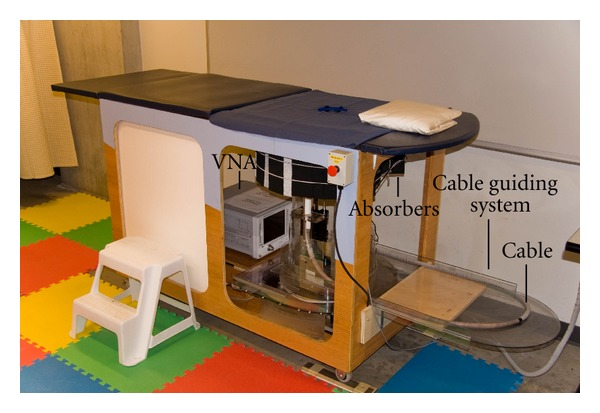
\includegraphics[width=0.5\textwidth]{TSARPrototype.png}
    \centering
    \caption{The TSAR Prototype \cite{bourquiPrototypeSystemMeasuring2012}}
    \label{fig:TSARPrototype}
\end{figure}

The benefit of the monostatic configuration is that the number of antenna locations per row and the number of rows are
parameters that can be tweaked depending on whether the radiologist would want a quicker scan or higher precision. One
can imagine the scenario of a rapid screening center as part of a national screening program where the speed of the scan
is valued over the precision of the scan. As such this provides a notable benefit over the previous two systems. The
clinical trial conducted by this study was extremely limited, only including 8 successfully imaged patients. Due to the
low sample size, one can't reliably say whether this system and its adaptive reflection-suppressing algorithm can
outperform the other two systems in terms of accuracy, although the TSAR system does show promise. \hfill 

\subsection{Beamformers}
Without loss of generality, imagine a line array of wave emitters. If all of these begin to emit at the same time, the
individual waves would constructively and destructively interfere with each other as their peaks and troughs align and
misalign. This property can be exploited in such a way so that the waves constructively interfere in one direction and
destructively interfere in all the other directions, effectively aiming the beam in a particular direction. A diagram
of this can be seen in Figure \ref{fig:phasedArray}.


\begin{figure}[!h]
    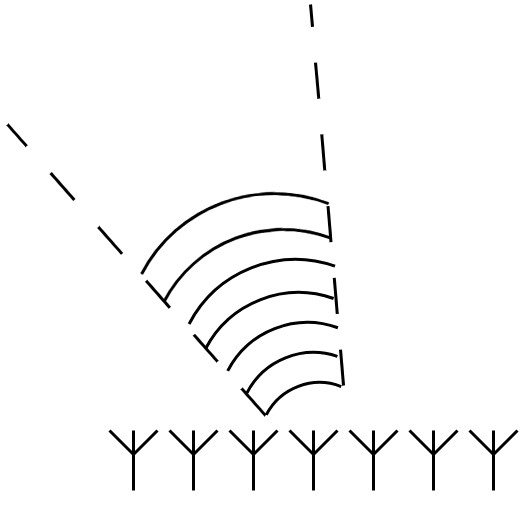
\includegraphics[width=0.5\textwidth]{phasedArray.png}
    \centering
    \caption{Phased Array Diagram}
    \label{fig:phasedArray}
\end{figure}

This is the forward beamforming process, but one can also consider the reverse process. Considering Figure \ref{fig:pointEmitter} imagine a point emitter
embedded in a 2D plane, that radiates circular waves evenly in all directions. Now imagine a line array that receives
this wave. Due to the diffusion of the wave through space, the same wave will appear at each antenna at different times. This would
manifest as the same amplitude appearing at different times, in the signal graphs, even though the impulses come from
the same wave. Reverse beamforming then, is the process of varying the phase and amplitude of the received signals in
order to estimate the intensity at the location where the wave originated. Inverse beamforming is a process used in many
fields such as radio astronomy and seismic imaging, so there already is a wealth of research and plenty of algorithms to
choose from. The rest of this section will talk about the various beamformers that are popular in the field of microwave
imaging. \hfill \break

\begin{figure}
    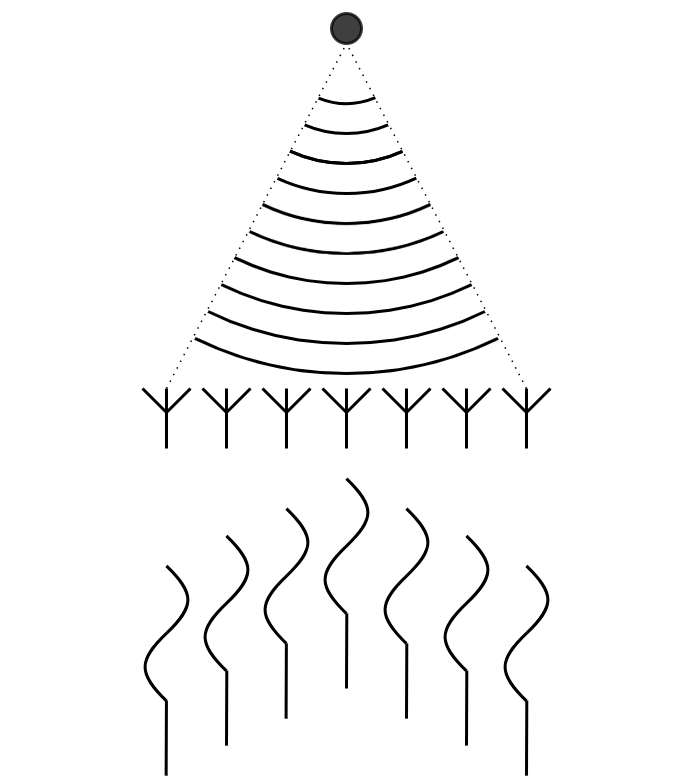
\includegraphics[width=0.6\textwidth]{pointEmitter.png}
    \centering
    \caption{Point Emitter with a Phased Array}
    \label{fig:pointEmitter}
\end{figure}

\subsubsection{Delay and Sum}
The Delay and Sum (DAS) beamformer is the template for most other beamforming algorithms in the field. The DAS
beamformer posits that every antenna has recorded the same source and that the delay in each signal is
due to the relative distance between the receiving antenna ($\mathcal{A}'$) and the transmitting antenna
($\mathcal{A}$). As such, if one was to delay the signals by the correct amount, and sum over all the received signals,
one would be able to estimate the energy at the source. This same idea can be applied to signals received from the
aforementioned imaging systems. Since these work in the frequency domain, the following explanations and equations will
work on this assumption, but these equations can easily be converted to the relative time domain functions. As stated
before a point from the imaging domain is chosen ($r$). We then estimate the path delay of the wave from the
transmitting antenna to the receiving antenna along the path.

\begingroup
\Large
\begin{equation}
    \tau_{\mathcal{A}_i', \mathcal{A}_j}(r) = \frac{\epsilon}{c_0} \left [\lVert \mathcal{A}' - r \rVert + \lVert r - \mathcal{A}\rVert\right ]
    \label{eq:PathDelayDAS}
\end{equation}
\endgroup


$\epsilon$ is the relative permittivity of the medium. In reality, this value changes from patient to patient and even
varies within the breast of each patient depending on the path taken. However in order to achieve a practical beamformer, one must estimate an
averaged relative permittivity value for the entire breast, we will label this as $\epsilon_i$ and it will parametrize
the DAS beamformer. As well as this, equation \ref{eq:PathDelayDAS} assumes a straight-line path between the point and
the transmitting and receiving antennas. This is rarely the case, however, in practice making this assumption
only yields a maximal error of 3mm in position while greatly simplifying the delay calculations
\cite{oloughlinParameterSearchAlgorithms2017}. Using this, the received signals are delayed and then summed across all
stepped input frequencies. This result is then squared to give us the energy at the chosen point. Thus the point is
imaged, This process is repeated for all the points in the imaging domain, overall the DAS beamforming equation can be
represented as such:

\begingroup
\Large
\begin{equation}
    I_{\epsilon_i}(r) = \left [\sum_{\Omega}\sum_{\mathcal{A}'}\sum_{\mathcal{A}} S_{a, a'}[\omega]e^{j\omega \tau_{\epsilon_i, a, a'}(r)}\right ]^2
    \label{eq:DASBeamformer}
\end{equation}
\endgroup

\subsubsection{Weighted Delay and Sum Beamformer}
The Weighted Delay and Sum (WDAS) Beamformer can be considered as a further generalization of the DAS beamformer.
In equation \ref{eq:DASBeamformer} all channels contribute equally to the final result due to the implicit weighting
factor of 1. The equation also assumes that all signals travel along similar paths, and therefore a constant speed (due
to the fixed $\epsilon_i$). In reality, this is only true for antennas that are closer together. The greater the
distance between the transmitting and receiving antennas, the greater the chance, that the waves deviate from the straight line
path, ergo the estimation of the speed and subsequently the delay along that path will be wrong. Essentially, the
algorithm needs to have some mechanism that would penalize the signal from antennas that are further away and reward
signals from antennas that are close by. This is what S.A. Shah Karam et al proposed in their 2021 paper, "Weighted delay-and-sum beamformer for breast cancer detection using
microwave imaging" \cite{shahkaramWeightedDelayandsumBeamformer2021}. They define a weighting factor based on the
transmitter-receiver distance ($TRD_i$) for
the $t^{th}$ observation:

\begin{equation}
    w_i = \alpha -  \lvert r_{T_{r_i}} - r_{R_{c_i}} \rvert
\end{equation}

In order to reward signals from antennas that are close and penalize antennas that are far away one must subtract the
$TRD_i$ from a positive constant, $\alpha$. This parameter is patient-specific and must be changed based on the homo- or
heterogeneity of the breast tissue. The paper used an $\alpha$ of 20cm for their results. One important thing to note is
that these weighting factors are data-independent. Since the $TRD_i$ relies only on the distance between the antennas,
these weighting factors can be computed beforehand. Another thing of note is that these weighting factors are
independent of the chosen focal point as well, which means we can compute a normalized weight and apply it to the signal
before employing the traditional DAS algorithm. The normalized weighting factor $\hat{w}_i$ is calculated as follows,
where $M$ is the number of channels:
\begin{equation}
    \hat{w}_i = \frac{w_i}{\sum_{i=0}^{M} w_i}
\end{equation} 

\subsubsection{Delay Multiply and Sum}
